\tikzset{every picture/.style={line width=0.75pt}} %set default line width to 0.75pt        

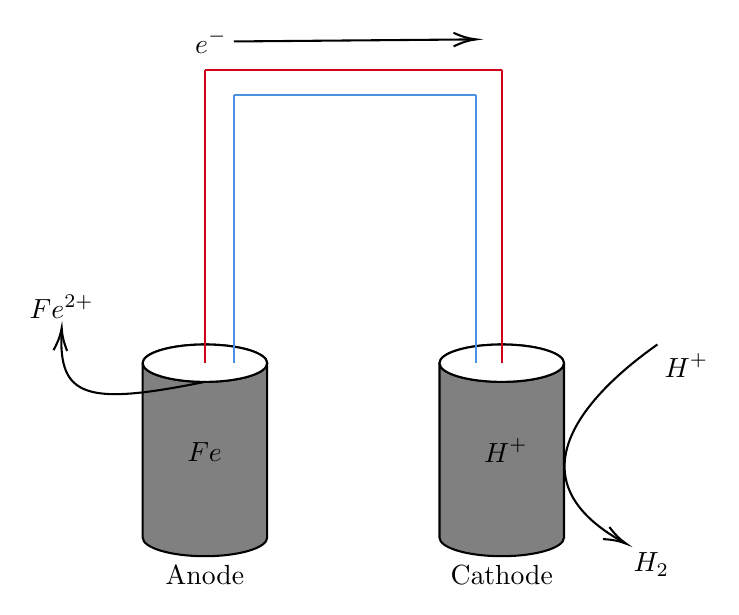
\begin{tikzpicture}[x=0.75pt,y=0.75pt,yscale=-1,xscale=1]
%uncomment if require: \path (0,300); %set diagram left start at 0, and has height of 300

%Shape: Can [id:dp4503664778559091] 
\draw  [fill={rgb, 255:red, 128; green, 128; blue, 128 }  ,fill opacity=1 ] (190,171) -- (190,255) .. controls (190,259.97) and (176.57,264) .. (160,264) .. controls (143.43,264) and (130,259.97) .. (130,255) -- (130,171) .. controls (130,166.03) and (143.43,162) .. (160,162) .. controls (176.57,162) and (190,166.03) .. (190,171) .. controls (190,175.97) and (176.57,180) .. (160,180) .. controls (143.43,180) and (130,175.97) .. (130,171) ;
%Shape: Ellipse [id:dp565979149570075] 
\draw  [fill={rgb, 255:red, 255; green, 255; blue, 255 }  ,fill opacity=1 ] (130,171) .. controls (130,166.03) and (143.43,162) .. (160,162) .. controls (176.57,162) and (190,166.03) .. (190,171) .. controls (190,175.97) and (176.57,180) .. (160,180) .. controls (143.43,180) and (130,175.97) .. (130,171) -- cycle ;
%Straight Lines [id:da3663451366147634] 
\draw [color={rgb, 255:red, 208; green, 2; blue, 27 }  ,draw opacity=1 ]   (160,29.58) -- (160,171) ;

%Shape: Can [id:dp0951927406661861] 
\draw  [fill={rgb, 255:red, 128; green, 128; blue, 128 }  ,fill opacity=1 ] (333,171) -- (333,255) .. controls (333,259.97) and (319.57,264) .. (303,264) .. controls (286.43,264) and (273,259.97) .. (273,255) -- (273,171) .. controls (273,166.03) and (286.43,162) .. (303,162) .. controls (319.57,162) and (333,166.03) .. (333,171) .. controls (333,175.97) and (319.57,180) .. (303,180) .. controls (286.43,180) and (273,175.97) .. (273,171) ;
%Shape: Ellipse [id:dp9301470966524585] 
\draw  [fill={rgb, 255:red, 255; green, 255; blue, 255 }  ,fill opacity=1 ] (273,171) .. controls (273,166.03) and (286.43,162) .. (303,162) .. controls (319.57,162) and (333,166.03) .. (333,171) .. controls (333,175.97) and (319.57,180) .. (303,180) .. controls (286.43,180) and (273,175.97) .. (273,171) -- cycle ;
%Straight Lines [id:da15512893440324627] 
\draw [color={rgb, 255:red, 208; green, 2; blue, 27 }  ,draw opacity=1 ]   (303,29.58) -- (303,171) ;

%Straight Lines [id:da5383287109318899] 
\draw [color={rgb, 255:red, 208; green, 2; blue, 27 }  ,draw opacity=1 ]   (160,29.58) -- (303,29.58) ;
%Straight Lines [id:da19199568942290224] 
\draw [color={rgb, 255:red, 74; green, 144; blue, 226 }  ,draw opacity=1 ]   (174,42) -- (174,171) ;
%Straight Lines [id:da8343730433897103] 
\draw [color={rgb, 255:red, 74; green, 144; blue, 226 }  ,draw opacity=1 ]   (290.6,42) -- (290.6,171) ;
%Straight Lines [id:da020014113786278376] 
\draw [color={rgb, 255:red, 74; green, 144; blue, 226 }  ,draw opacity=1 ]   (290.6,42) -- (174,42) ;
%Curve Lines [id:da7591506959538374] 
\draw    (378,162) .. controls (351.14,180.91) and (301.5,224.56) .. (362.08,257.5) ;
\draw [shift={(363,258)}, rotate = 208.02] [color={rgb, 255:red, 0; green, 0; blue, 0 }  ][line width=0.75]    (10.93,-3.29) .. controls (6.95,-1.4) and (3.31,-0.3) .. (0,0) .. controls (3.31,0.3) and (6.95,1.4) .. (10.93,3.29)   ;
%Curve Lines [id:da17504057504299442] 
\draw    (160,180) .. controls (102.18,191.76) and (89.5,187.19) .. (90.9,155.95) ;
\draw [shift={(91,154)}, rotate = 453.47] [color={rgb, 255:red, 0; green, 0; blue, 0 }  ][line width=0.75]    (10.93,-3.29) .. controls (6.95,-1.4) and (3.31,-0.3) .. (0,0) .. controls (3.31,0.3) and (6.95,1.4) .. (10.93,3.29)   ;
%Shape: Boxed Line [id:dp5443668674906494] 
\draw    (174,16) -- (288.71,15.02) ;
\draw [shift={(290.71,15)}, rotate = 539.51] [color={rgb, 255:red, 0; green, 0; blue, 0 }  ][line width=0.75]    (10.93,-3.29) .. controls (6.95,-1.4) and (3.31,-0.3) .. (0,0) .. controls (3.31,0.3) and (6.95,1.4) .. (10.93,3.29)   ;

% Text Node
\draw (150,208) node [anchor=north west][inner sep=0.75pt]   [align=left] {$\displaystyle Fe$};
% Text Node
\draw (380,165) node [anchor=north west][inner sep=0.75pt]   [align=left] {$\displaystyle H^{+}$};
% Text Node
\draw (293,206) node [anchor=north west][inner sep=0.75pt]   [align=left] {$\displaystyle H^{+}$};
% Text Node
\draw (91,151) node [anchor=south] [inner sep=0.75pt]   [align=left] {$\displaystyle Fe^{2+}$};
% Text Node
\draw (172,16) node [anchor=east] [inner sep=0.75pt]   [align=left] {$\displaystyle e^{-}$};
% Text Node
\draw (160,267) node [anchor=north] [inner sep=0.75pt]   [align=left] {Anode};
% Text Node
\draw (303,267) node [anchor=north] [inner sep=0.75pt]   [align=left] {Cathode};
% Text Node
\draw (365,261) node [anchor=north west][inner sep=0.75pt]   [align=left] {$\displaystyle H_{2}$};


\end{tikzpicture}
